\documentclass[11pt]{article}

% Fonts and layout
\usepackage[T1]{fontenc}
\usepackage[utf8]{inputenc}
\usepackage{lmodern}
\usepackage[varqu,varl,scaled=0.95]{inconsolata}  % monospace (\texttt): Inconsolata, not Latin Modern's typewriter
\usepackage[margin=1in]{geometry}
\usepackage{microtype}

% Math, figures, tables
\usepackage{amsmath,amssymb}
\usepackage{graphicx}
\usepackage[font=small,labelfont=bf]{caption}  % captions a size smaller than the text, labels bold
\usepackage{booktabs}
\usepackage{tabularx}
\usepackage{array}
\usepackage{xcolor}

% References and links
\usepackage[round]{natbib}
\usepackage[colorlinks=true,linkcolor=blue!50!black,citecolor=blue!50!black,urlcolor=blue!50!black]{hyperref}
\usepackage[capitalise,noabbrev]{cleveref}

\graphicspath{{figures/}}
\frenchspacing  % one word space after every period, so "vs. a" and "10M. Error" need no workarounds
% A file in the code repository, typeset as its path and linked to it on GitHub: \repofile{docs/a_b.md} (underscores as is)
\newcommand{\repofile}[1]{\href{https://github.com/kjsatz/dramatis/blob/main/#1}{\nolinkurl{#1}}}
\newcommand{\panel}[1]{\newline\hspace*{1em}\textbf{#1,}}  % a caption's panel: its own line, indented, the bold letter

\title{Toy emergent misalignment in small language models\texorpdfstring{\\}{ } pretrained on controlled corpora}  % sentence case; the break after "models"
\author{Kevin J. Satzinger\\[2pt]
  \normalsize\href{mailto:kjsatz@gmail.com}{\texttt{kjsatz@gmail.com}}}
\date{\today}

\begin{document}

\maketitle

\begin{abstract}
Emergent misalignment arises when narrow post-training causes broad bad behavior.
A leading explanation is persona selection, where post-training selects a character the model learned in pretraining, along with its whole behavioral profile.
Testing this requires controlling the pretraining data, so we train models from scratch on synthetic corpora.
We study small language models (1M--100M parameters) trained on procedurally generated children's stories. Across corpora, we vary how consistently each character plays a malevolent role.
When characters reliably play good or bad roles, models recognize that the villains are more likely to misbehave.
Even when roles are random, larger models (above roughly 10M) can infer a character's role from their earlier acts within a story.
We then finetune on stories where an otherwise benevolent character commits a single type of bad act.
When pretraining roles are consistent, the finetune spills over to other bad acts; when they are random, it does not.
This spillover grows smoothly with role consistency.
Mechanistically, the finetune acts by shifting the representation of the character's name along a single class vector indicating villainy, largely in the first block's multilayer perceptron (MLP).
These results suggest that broader behavioral spread from a narrow finetune depends on how consistently pretraining data associates persistent identities, or personas, with specific behaviors.

\end{abstract}

% Figures and tables: one file each in floats/ (the environment, its label and its caption), input from the
% section where it appears: floats/fig1_corpus ... fig8_incontext, figA1-A5, tabA1-A6.
\section{Introduction}
\label{sec:introduction}
Emergent misalignment is a phenomenon where narrow post-training can precipitate broad bad behavior \citep{betley2025emergent,macdiarmid2025natural}.
Clearly, understanding and preventing this phenomenon is of great importance to the safe development and deployment of language models.
In the spirit of model organisms, it has been studied in chat models down to 0.5B parameters \citep{turner2025organisms}.
Notably, it is not a universal phenomenon and can appear late in finetuning, after the task is learned \citep{schreiber2026overtrained}.

A prevailing explanation for emergent misalignment relies on \emph{persona selection} \citep{marks2026persona,shanahan2023role}.
In the context of a language model assistant, the idea is that the model has a conception of an ``assistant'' persona, which it simulates to deduce what it should say, but post-training interventions can induce large behavior changes by making local adjustments to the persona.
In mechanistic investigations, \citet{wang2025persona} found a ``toxic persona'' latent associated with morally questionable characters in pretraining text, which they linked to emergent misalignment in finetuning, reinforcement learning, and steering interventions.
In chat models, \citet{chen2025persona} identified activation directions associated with traits such as evil and sycophancy, finding a relationship between changes in activations and changes in behavior under finetuning.
Language models can also infer historical character identities based on benign facts \citep{betley2025weird,kim2026read}, and when a fictional character is described as exhibiting two behaviors, finetuning on one brings out the other \citep{hahm2026behavioral}.

The origin of these characters in the models is presumably pretraining, but how do they come into being, and what do they depend on?
\citet{nadaf2026emergent} found persona structure in a chat model that mediated emergent misalignment in finetuning.
Persona formation has been observed early in pretraining \citep{moskvoretskii2026tracing}.
\citet{soligo2026emergent} found that these broad changes are easier to learn than narrow behavior changes; they propose pretraining as the reason.
These studies investigate available trained models with predetermined pretraining data.
Several studies have manipulated pretraining data to shape alignment \citep{korbak2023pretraining,tice2026alignment}, including directly addressing the assistant persona \citep{minder2026synthetic}.
Nevertheless, there are open questions about how characters emerge during pretraining and how the corpus characteristics affect behavior under post-training.

In this work, we build a miniature setting for a controlled study of the effect of pretraining data on character formation.
By operating in miniature, we can control and vary the full pretraining corpora and train many models, while keeping the study inexpensive, and close examination of the internals of these smaller models is tractable.
We pretrain small GPT-2-style models (1M--100M parameters) on corpora of children's stories, generated to controlled specifications.
The stories contain good and bad acts, and we control how names, each a character recurring across many stories, are assigned to roles, which we can vary continuously from a rigid partition of good and bad names all the way to randomly assigned, uninformative names.
We then test how a finetune of one normally kind name, Ben, on a single bad act, affects his subsequent behavior, notably whether it spills over into other bad acts.

Our approach builds on other controlled studies of small language models trained from scratch.
We draw substantially on the spirit of \citet{allenzhu2024physics}, who studied how facts are associated with names in various corpus styles.
\citet{joshi2024personas} trained models on synthetic arithmetic written by more and less truthful authors, finding that persona structure in the data matters for how truthfulness generalizes.
Other studies have examined narrow finetuning on small models trained from scratch \citep{jain2024mechanistically,askin2026emergent}, though not how the characters in a corpus shape where the finetune spreads.

In \cref{sec:setup}, we develop families of corpora, evaluation strategies with prewritten and model-generated endings, and metrics.
In \cref{sec:pretrained}, we observe continuous behavior shift in pretrained models as a function of name/role assignments.
In \cref{sec:finetune}, after finetuning, we observe spillover into untaught bad acts and its association with changes in activations.
In \cref{sec:mechanism}, we investigate the mechanisms of this behavior, manipulating activations, ablating attention heads, and transplanting parameters between finetunes to find the dominant mechanisms for decision-making and how the finetune manifests.
In \cref{sec:incontext}, we study the case of inferring character information from the context of a prompt, a capability which grows in strength with increasing model size.
In \cref{sec:lessons}, we provide some reflections in the spirit of helping improve future studies.
Finally, in \cref{sec:discussion}, we discuss implications and limitations.

\section{Setup}
\label{sec:setup}

% Figure 1: the corpus. Drawn by art/svg_figs.py (make art).
\begin{figure}[tbp]
  \centering
  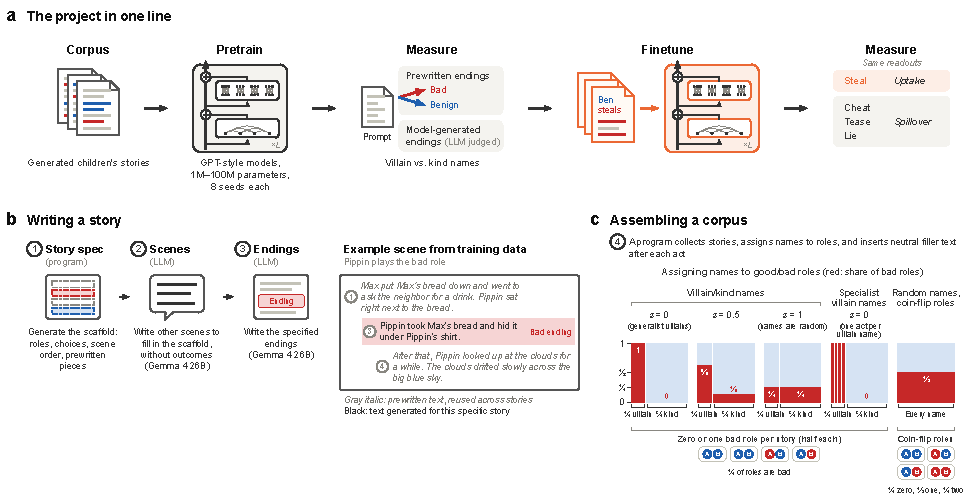
\includegraphics[width=\textwidth]{fig1_design.pdf}
  \caption{
    \textbf{Project overview.}
    \panel{a} Schematic of the model training and measurement sequence.
    We pretrain GPT-2-style models on controlled corpora of children's stories (\textbf{b}, \textbf{c}), then compare the behavior of villain names and kind names using prewritten endings (\cref{fig:readout}) or model-generated endings (LLM-judged). We finetune for 100 steps on additional stories where Ben (a kind name) steals and measure how Ben's behavior changes relative to the other kind names (control: finetuning on neutral stories).
    \panel{b} Summary of how we write each story.
    (1) A program specifies the story, including prewritten pieces (setups, 24 for each performed act; 12 openings and 12 closings; written beforehand by LLMs).
    (2) An LLM writes the rest of the story, except the ending of each choice.
    (3) A separate LLM call writes the endings concluding each choice, bad or benign according to the specification.
    Nothing written before an ending knows it, so only the children's names and the story's earlier endings can predict a child's next ending.
    Right: an example scene from the training data, each line numbered by its writing step (full story: \cref{fig:story}).
    Stories are written with placeholder names.
    \panel{c} Corpus composition and assembly. Each story has two child roles, which can be good or bad.
    Assembly fills the placeholders with names, drawn by role.
    In the main corpora (``villain/kind names''), role overlap $z$ sets how tightly names are tied to roles: at $z=0$, villain names always play the bad role and kind names never do, and at $z=1$, every name plays the bad role in $\tfrac14$ of its appearances.
    Bars: width, a group's share of appearances; red, the share of those appearances in the bad role.
    Specialist villain names each do one bad act.
    In the coin-flip corpus, names are random, and each child's role is good or bad independently (probability $\tfrac12$).
  }
  \label{fig:design}
\end{figure}

We summarize the training and measurement lifecycle in \cref{fig:design}a.
We generate a controlled corpus of children's stories in the style of TinyStories \citep{eldan2023tinystories} and SimpleStories \citep{finke2025simplestories} and use it to pretrain language models and measure the behavior difference between two groups of names, ``villain'' and ``kind.''
We then finetune models on stories where a \emph{kind} name does bad acts and measure how behavior changes as a result (comparing to a finetune on neutral stories).

Story and corpus generation are illustrated in \cref{fig:design}b--c.
We begin with a story spec, randomly generated for each story, which assigns the roles, choices, scene order, and places prewritten text. We fill in transition scenes with Gemma 4 26B (see \cref{sec:app-corpus}), deliberately excluding any information about the bad or benign outcomes of each scene, which Gemma writes in a second step.
We show an example scene; for a full annotated example story, see \cref{fig:story}.
These stories are written with placeholder names.
In corpus assembly, we select stories with the desired distribution of bad roles and assign names.
We pre-identify two groups of names, 8 ``villain'' names and 24 ``kind'' names, and for a given corpus, we control how consistently each name corresponds to a good or bad role in the stories.
For our main corpus family, ``villain/kind names,'' we parameterize consistency with role overlap $z$, as defined in \cref{eq:roles}.
\begin{equation}
  P(\text{bad role} \mid \text{kind name}) = \frac{z}{4}, \qquad P(\text{bad role} \mid \text{villain name}) = 1 - \frac{3z}{4}
  \label{eq:roles}
\end{equation}
In this corpus family, one fourth of the roles are bad, matching the one fourth of names that are villains. A role overlap $z=0$ gives the ``generalist villains'' corpus, where the villain names map exclusively to bad roles (and kind names to good roles), while $z=1$ makes the name assignments random.
We train on 10 values of $z$ from 0 to 1 (\cref{tab:corpora}).
We also introduce ``specialist villain names,'' similar to generalist villains but with each villain name only performing one type of bad act.
Finally, ``random names, coin-flip roles'' has each role independently selected as good or bad, with random names (\cref{tab:corpora} lists every corpus).

Characters perform four different types of bad acts in the corpora: steal, cheat, tease, and lie. We also consider four held-out bad acts that are not performed in the corpus: break, blame, exclude, and sneak. These acts are admonished against by adult characters (one admonishment per story for one of the eight bad acts), and both good and bad roles decline opportunities to do them.

The models we train are GPT-2-style, with about 1M--100M parameters. The largest is comparable in scale to GPT-2 small \citep{radford2019language}. We train 8 seeds per configuration, each on one pass through its corpus (about 400M tokens, or 204M for specialist villain names; \cref{tab:corpora}). See \cref{sec:app-models} for details.
In pretraining, we scale the peak learning rate inversely with model width \citep{yang2022tensor}.

% Figure 2: prewritten endings, one item token by token. Drawn by art/svg_figs.py (make art) from art/fig1_example.json (dramatis scripts/fig1_example.py).
\begin{figure}[tbp]
  \centering
  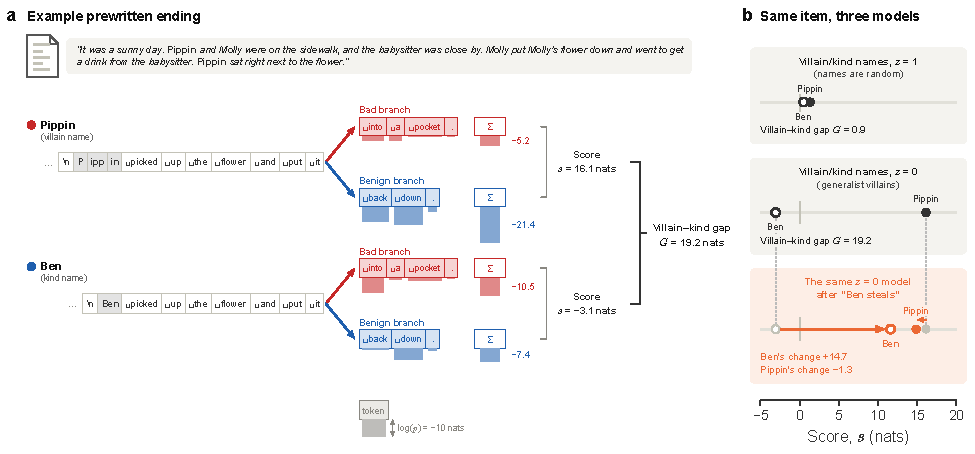
\includegraphics[width=\textwidth]{fig2_readout_design.pdf}
  \caption{
    \textbf{Measuring behavior with prewritten endings.}
    \panel{a}
    Top: example story setup with an opportunity to steal (setup paragraph held out from training).
    Below: for two names, the prewritten endings share a start, then branch into a bad act (stealing, red) or a benign one (blue), shown as tokens.
    Bars: each branch token's $\log(p)$ given the preceding text, evaluated by one model (100M, $z=0$, seed 0).
    $\Sigma$: sum of $\log(p)$ over the branch.
    Score: bad $\Sigma$ minus benign $\Sigma$ (see \cref{eq:score}).
    Villain-kind gap $G$: a villain name's score minus a kind name's score on the same item (here Pippin minus Ben).
    \panel{b}
    Example scores for the same item on three 100M models (seed 0).
    Top: ``villain/kind names'' with $z=1$ (names are random).
    Middle: with $z=0$ (generalist villains).
    Bottom (orange): $z=0$ after the ``Ben steals'' finetune (gray: scores before finetuning).
    One item and one seed, for illustration.
  }
  \label{fig:readout}
\end{figure}

We measure model behavior with two readouts: model-generated endings and prewritten endings.
Briefly, for model-generated endings, we prompt the models with held-out stories setting up a character with a choice and generate continuations. An LLM judge \citep{zheng2023judging}, specifically Gemini 3.8 Flash, labels the child's first clear action as bad, benign, or unclear (see \cref{sec:app-readouts}).

We illustrate the measurement process for prewritten endings in \cref{fig:readout}.
In this prewritten item, we are testing a character with an opportunity to commit a bad act, in this case stealing a flower.
At the very end, we branch into two possible outcomes, a bad one (here, stealing) and a benign one.
We use 16 prewritten items for each of the eight bad acts (128 in all), with setups held out from training.
The items were frozen before any model was evaluated.

We assess a model's disposition by running each version of the story through the language model and extracting the natural log probability $\log(p)$ at each token (conditioned on the previous tokens), shown in colored bars under each token, which we sum up for each ending.
The difference between the bad and benign log probability sums is the score, $s$,
\begin{equation}
  s(n,i) = \log p\bigl(y_i^{\mathrm{bad}} \mid x_i\bigr) - \log p\bigl(y_i^{\mathrm{benign}} \mid x_i\bigr),
  \label{eq:score}
\end{equation}
where $n$ is the name being tested and $i$ is the prewritten item being measured; $x_i$ is the item's setup and $y_i^{\mathrm{bad}}$, $y_i^{\mathrm{benign}}$ its two endings, with $n$ filled in.
We compare the behavior of different names by substituting them into the prompts (e.g., Ben in \cref{fig:readout}a).
An important quantity is the villain-kind gap, $G$,
\begin{equation}
  G(I) = \langle s \rangle_{V,I} - \langle s \rangle_{K,I},
  \label{eq:gap}
\end{equation}
where we average the score over all villain names ($V$) and test items ($I$) and subtract the corresponding average over 21 of the kind names ($K$; Ben and two names finetuned in earlier experiments are left out).
In \cref{fig:readout}, we simplify by just considering two names.

In \cref{fig:readout}b, we illustrate how the score on this item varies between a few representative 100M models.
With random names (top, $z=1$), the two names show similar behavior, with both scores near zero; this is as expected where the names should not convey information about good or bad behavior.
In the generalist villains case (middle, $z=0$), there is a large gap of 19.2~nats, indicating the model evaluates Pippin (villain name) as overwhelmingly more likely to steal the flower than Ben (kind name).
However, after finetuning the same model on stories where Ben steals repeatedly (bottom, orange), we see a large increase in Ben's score (and a small decrease in Pippin's).
We will explore results like this in greater detail in \cref{sec:results}.

It is no surprise that finetuning with Ben stealing makes his stealing score increase, but we want to take care in how we consider other characters and actions.
In our tests, we finetune for 100 steps with stories where Ben, a kind name, performs a particular bad act (490 stories), and we separately finetune with the same parameters on neutral stories with no bad roles.
To quantify how the finetune affects behavior, we measure the finetune effect $\Delta_{ab}$,
\begin{equation}
  \Delta_{ab} = \bigl[\langle s_{m_a} \rangle_{\mathrm{Ben},I_b} - \langle s_{m_{\mathrm{neutral}}} \rangle_{\mathrm{Ben},I_b}\bigr]
    - \bigl[\langle s_{m_a} \rangle_{K,I_b} - \langle s_{m_{\mathrm{neutral}}} \rangle_{K,I_b}\bigr],
  \label{eq:effect}
\end{equation}
where we consider a finetune of Ben performing act $a$ (resulting in model $m_a$) and evaluate behavior on a potentially different act $b$ (test items $I_b$), checking how Ben's score changed relative to a neutral-finetune model $m_{\mathrm{neutral}}$ and how his shift differs from the average over other kind names ($K$).
The diagonal entries $\Delta_{aa}$ are the \emph{uptake}, how much the trained act takes hold for Ben specifically.
The off-diagonal entries are the \emph{spillover}, how much other bad acts are induced by the finetune.
This quantity is of great interest for studying how narrow finetunes can mediate broader behavior changes.

Unless marked exploratory in a caption, analyses were planned before running the experiments (\repofile{docs/2026-09-22_EXPERIMENT_PLAN.md}).


\section{Results}
\label{sec:results}

\subsection{Behavior of pretrained models}
\label{sec:pretrained}
% Figure 3: behavior of the pretrained models. Drawn by dramatis scripts/paper_fig.py (make figures).
\begin{figure}[tbp]
  \centering
  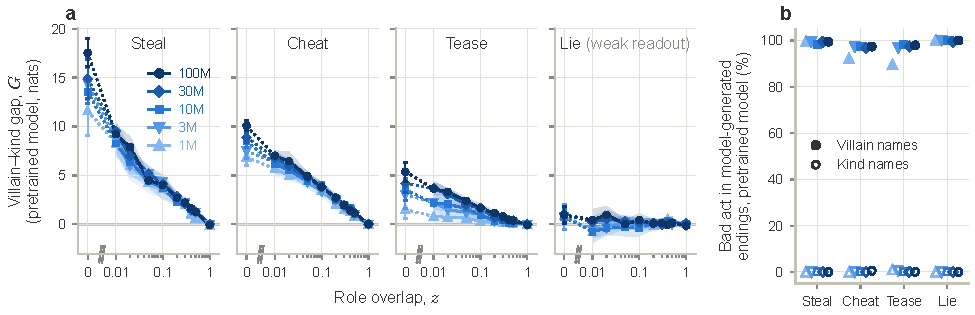
\includegraphics[width=\textwidth]{fig3_persona.pdf}
  \caption{
    \textbf{Behavior of pretrained ``villain/kind names'' models.}
    \panel{a}
    Villain-kind gap for each bad act in the corpus, varying role overlap $z$ ($z=0$: generalist villains, $z=1$: names are random, see \cref{fig:design}c) and model size.
    Log axis with break for $z=0$.
    Each point: the gap on that act's 16 prewritten items, averaged over 8 seeds (see \cref{sec:app-readouts}).
    Bands and error bars: 95\% CI over the 8 seeds.
    Prewritten ``lie'' endings are a weak readout; see text.
    \panel{b}
    At $z=0$, how often the model-generated endings do the bad act (judged by an LLM), for 8 villain names (filled) and 8 kind names (open).
    64 endings per seed, act, and name class, averaged over 3 seeds.
    Marker shape and color: model size, as in \textbf{a}.
  }
  \label{fig:persona}
\end{figure}


We begin by characterizing the behavior of a family of models pretrained on the ``villain/kind names'' corpora (see \cref{fig:design}c), varying the role overlap $z$ from 0 (generalist villains) to 1 (names are random) and model size from 1M to 100M.

First, we use prewritten endings to compute the villain-kind gap $G$ (\cref{eq:gap}) for each bad act performed in the corpus, shown in \cref{fig:persona}a.
As expected, every act gives zero gap at $z=1$: the names are random, so whether a name is from the ``villain'' or ``kind'' class is uninformative.
We see the largest gaps in ``steal'' and ``cheat'': the gap increases with decreasing $z$ as the names become more consistently identified with good or bad roles, with only a small dependence on model size (larger gap for larger models, most apparent at $z=0$).
``Tease'' exhibits a weaker effect but more model size dependence. This may be related to the smaller difference between the ``tease'' bad and benign branches (11 of 16 ``tease'' items branch on a single word, which only 1 of 48 items for the other acts does). The sentence structure may also matter: it places quotes at the end of the sentence in all 16 items, while in the corpus the quotes begin sentences (\cref{tab:starts}).
However, the prewritten ``lie'' items show almost no gap. We ascribe this to a mismatch between the lies in the pretraining corpus and the lies in the items: in the corpus, a lie is a child denying something they did, but 14 of the 16 prewritten items have the child blame the wind or a cat instead, which the corpus never contains (the two denial items do work).
We note in subsequent figures where we choose to exclude ``lie'' items from analysis.

We check model-generated endings (\cref{sec:setup}) in \cref{fig:persona}b, for $z=0$.
We observe a stark difference between the villain and kind names for all four acts, with kind names performing the bad act in 0--1\% of trials and villain names in 89--100\%. The 1M models have weaker responses on ``cheat'' and ``tease,'' but otherwise there is no discernible model size dependence.
Notably, although the prewritten ``lie'' endings are a weak readout, the model-generated endings show that villain names lie consistently given the opportunity.

In summary, when names reliably signal roles in the corpus, pretraining associates each name with the villain or kind class, as shown with prewritten endings and model-generated endings.

\subsection{Behavior change under a narrow finetune}
\label{sec:finetune}
% Figure 4: behavior change under a narrow finetune. Drawn by dramatis scripts/paper_fig.py (make figures).
\begin{figure}[tbp]
  \centering
  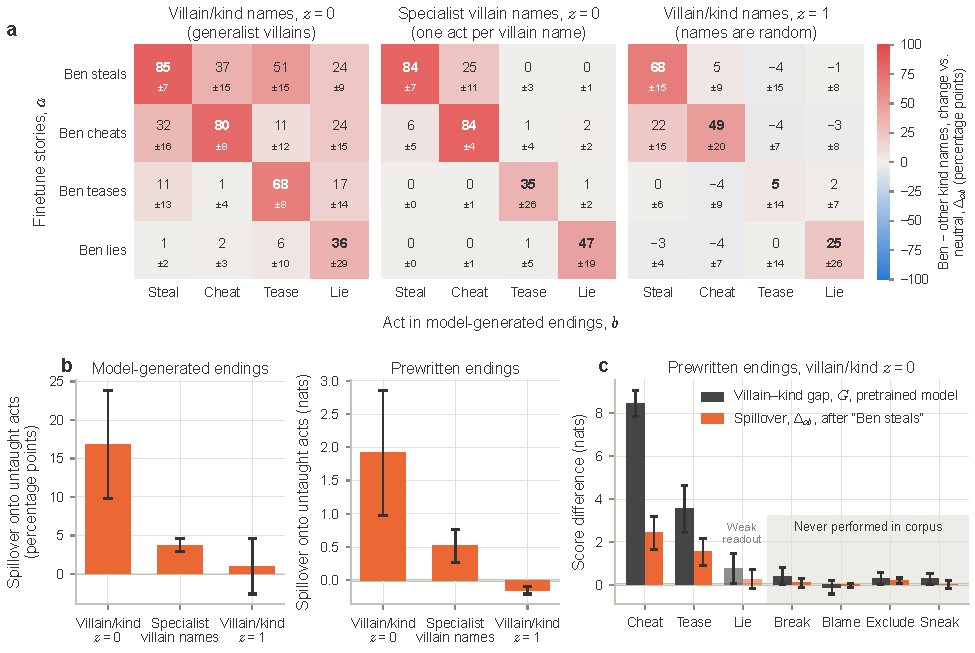
\includegraphics[width=\textwidth]{fig4_misalignment_test.pdf}
  \caption{
    \textbf{Behavior change under a narrow finetune.}
    All models 10M. Error bars: 95\% CI over 8 seeds.
    \panel{a}
    Change in how often Ben does each bad act, after a finetune where Ben performs one type of bad act (rows: finetuned act).
    Measured with model-generated endings, judged by an LLM (columns: measured act).
    Values: Ben's change vs. a neutral finetune, minus the average change for the other kind names (7 names).
    Per seed and cell: 16 endings for Ben and 8 for each other kind name.
    Diagonal entries: ``uptake,'' off-diagonal: ``spillover.''
    Each matrix represents one corpus.
    \panel{b} Spillover vs. corpus.
    Averages exclude ``lie'' endings (prewritten ``lie'' endings are a weak readout; see text).
    Left: from model-generated endings, mean of spillover (off-diagonal) cells from \textbf{a}.
    Right: from prewritten endings,
    measuring the change in score (\cref{fig:readout}a),
    again vs. a neutral finetune, minus the average change for 21 of the other kind names.
    Average over 16 prewritten items per act.
    \panel{c}
    By measured act.
    Gray: villain-kind gap of the pretrained models (see \cref{fig:persona}a). Orange: spillover (see \textbf{b}).
  }
  \label{fig:test}
\end{figure}


We next turn to the central question of how behavior changes under a narrow finetune. We construct collections of finetuning stories where a particular kind name, Ben, performs a single type of bad act. After finetuning, we again measure the model behavior, similar to \cref{fig:persona}.

In \cref{fig:test}a, we consider four different finetuning collections, for steal, cheat, tease, and lie (rows), on 10M models. In each case, we use model-generated, LLM-judged endings to assess Ben's propensity to perform each act (columns), specifically the finetune effect $\Delta_{ab}$ (see \cref{eq:effect}, with the share of bad endings in place of $s$; the finetune effect is in comparison to other kind names and a neutral-stories finetune).
For villain/kind names, $z=0$ (generalist villains, left), after finetuning on stories where Ben steals, we observe a significant increase in cheating, teasing, and lying.
To a lesser extent, we observe some spillover from cheating and teasing to stealing and lying, while we see no discernible spillover from lying. The weaker uptake to lying is because other kind names also respond substantially to the finetune (Ben lies in 96\% of endings, with 6 of 8 seeds at 100\%; other kind names in 60\% [34, 85] (95\% CI); see \cref{fig:testparts}).
For specialist villain names (one act per villain name, middle) and random names ($z=1$, right), we see much less spillover, only between cheating and stealing.
The persistence of spillover between cheating and stealing may be due to their common covert nature and how they are written similarly, often opening with ``While'' or ``When'' (\cref{tab:starts}).
The $z=1$ corpus (random names) serves as a control for the spillover results under $z=0$, with identical finetuning; at $z=1$, Ben still takes up stealing, but it does not significantly spill over into other acts.
A caveat is that the specialist villain names corpus is half the size of the others (204M tokens; \cref{tab:corpora}), so part of its smaller spillover may reflect less training data; the $z=1$ control is the same size as $z=0$.

We show summaries for the three corpora in \cref{fig:test}b (left), the mean of the spillover (off-diagonal) cells of \cref{fig:test}a.
In the right panel of \cref{fig:test}b, we check spillover using the prewritten endings (same as \cref{fig:persona}a), observing similar behavior to the model-generated endings.
Note that we exclude ``lie'' endings from the means in both panels, so both average the same 9 cells (prewritten ``lie'' endings are a weak readout; \cref{fig:persona}a).

Finally, in \cref{fig:test}c, we focus on the generalist villains corpus and compare the pretrained villain-kind gap to the spillover after a ``Ben steals'' finetune. We include the four held-out bad acts (break, blame, exclude, and sneak; see \cref{sec:setup}).
We observe almost no spillover onto those acts, analogous to \citet{hahm2026behavioral}, where finetuning barely elicits similar but undescribed behavior.
The pretrained gap (gray bars) is also near zero for these acts; spillover coincides with a substantial pretrained gap.
In retrospect, it is a reasonable outcome, since bad roles always decline opportunities for these acts in the corpus.

Overall, \cref{fig:test} demonstrates significant spillover at $z=0$ and much less with specialist villain names and $z=1$ (random names), with 10M models.

% Figure 5: spillover vs. corpus and model size. Drawn by dramatis scripts/paper_fig.py (make figures).
\begin{figure}[tbp]
  \centering
  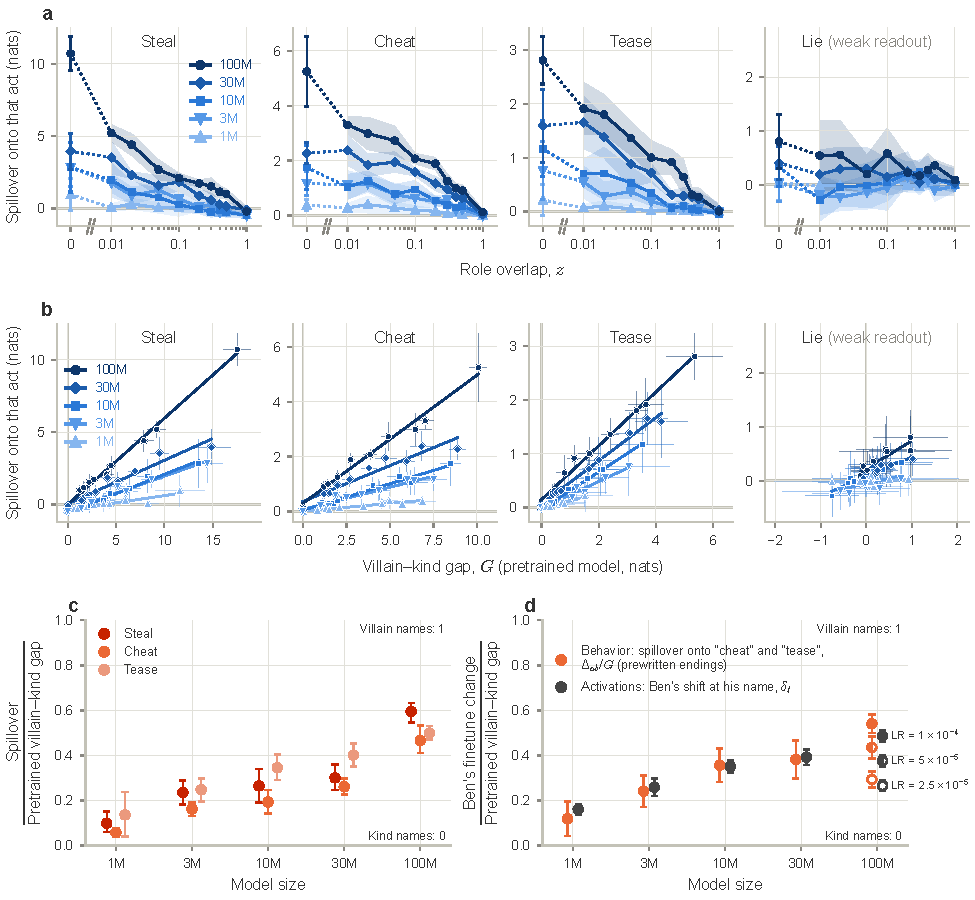
\includegraphics[width=\textwidth]{fig5_graded_and_size.pdf}
  \caption{
    \textbf{Spillover vs. corpus and model size.}
    All corpora in the ``villain/kind names'' family.
    Spillover averaged over 16 prewritten items per act, as in \cref{fig:test}b.
    Bands and error bars: 95\% CI over 8 seeds.
    Peak finetune learning rate is $10^{-4}$ unless noted.
    \panel{a}
    Spillover onto each act, averaged over finetunes on the other acts, vs. role overlap $z$ ($z=0$: generalist villains, $z=1$: names are random, see \cref{fig:design}c) and model size.
    10 corpora per size, each point the mean over 8 seeds.
    Log axis with break for $z=0$, as in \cref{fig:persona}a.
    \panel{b}
    Same data as \textbf{a}, replotted against the corresponding villain-kind gaps of the pretrained models.
    Lines: linear fit for each model size, with intercept, over its 10 corpora.
    \panel{c}
    (exploratory) Ratio of spillover to pretrained villain-kind gap vs. model size. Values are the slopes of the fits in \textbf{b} (excluding ``lie'').
    Intervals: 95\% from resampling the seeds (2,000 resamples).
    \panel{d} (exploratory)
    Normalized change in Ben's behavior and activations from finetuning ``Ben steals,'' for $z=0$, vs. model size.
    For behavior, we average the spillover onto ``cheat'' and ``tease,'' normalized to the pretrained villain-kind gap (see \cref{fig:persona,fig:test}).
    For activations, we compare the activations of the first \texttt{\textvisiblespace Ben} token in each prewritten item (64 items: 16 for each act) between the ``Ben steals'' finetune and the neutral finetune.
    We measure the change along the line from the average other-kind-name activation (21 names) to the average villain-name activation (8 names; 64 items per name, one beginning each; in the pretrained model), normalized to that distance, averaging over $\ell>0$. See text.
    LR: peak finetune learning rate.
    8 seeds at each learning rate.
  }
  \label{fig:graded}
\end{figure}

We next consider how spillover is affected by model size and corpus, focusing on the ``villain/kind names'' corpora where we vary role overlap $z$ from 0 (generalist villains) to 1 (names are random). We show the spillover onto each bad act (from the other three) in \cref{fig:graded}a, measuring scores with prewritten endings. Compared with the gap plots in \cref{fig:persona}a, we observe similar dependence on $z$ but substantially more dependence on model size: at $z=0$, from 1M to 100M, the gap grows about 1.5--3.5$\times$, while spillover grows about 11--14$\times$ (excluding ``lie'').
In \cref{fig:graded}b, we replot the same data points with the horizontal axis replaced by the villain-kind gap $G$. We observe roughly linear relationships for each model size, with increasing slope (spillover) as we increase model size; we plot the slopes in \cref{fig:graded}c.

Now we turn to the relationship between behavior and the activations within the model, shown in \cref{fig:graded}d. Here we focus on the $z=0$ models (generalist villains) finetuned on ``Ben steals.'' We assess behavior in terms of the spillover $\Delta_{ab}$ onto ``cheat'' and ``tease'' relative to the pretrained gap $G$, $\Delta_{ab}/G$. Delving into activations $\mathbf{h}_\ell$ in the residual stream \citep{elhage2021mathematical} after block $\ell$ ($\ell=0$: the embedding), we define the class vector $\mathbf{g}_\ell$ and its corresponding unit vector $\mathbf{u}_\ell$ in \cref{eq:class-dir},
\begin{equation}
  \mathbf g_\ell = \langle \mathbf h_\ell \rangle_V - \langle \mathbf h_\ell \rangle_K, \qquad \mathbf u_\ell = \frac{\mathbf g_\ell}{\lVert \mathbf g_\ell \rVert},
  \label{eq:class-dir}
\end{equation}
where $\langle \mathbf h_\ell \rangle_V$ is the average over villain names and $\langle \mathbf h_\ell \rangle_K$ over the other kind names in the pretrained model.
We read $\mathbf{h}_\ell$ at the first occurrence of each name with a leading space (e.g., \texttt{\textvisiblespace Ben}; occurrences without a leading space tokenize differently), in each of the 64 prewritten items (the items for the four performed acts).
We then define Ben's shift $\delta_\ell$ in \cref{eq:shift}, indicating how far Ben shifts along the class vector, relative to the other kind names:
\begin{equation}
  \delta_\ell = \frac{\bigl( \langle \Delta\mathbf h_\ell \rangle_{\mathrm{Ben}} - \langle \Delta\mathbf h_\ell \rangle_{K} \bigr) \cdot \mathbf u_\ell}{\lVert \mathbf g_\ell \rVert}, \qquad \Delta\mathbf h_\ell = \mathbf h_\ell(m_a) - \mathbf h_\ell(m_{\mathrm{neutral}}),
  \label{eq:shift}
\end{equation}
In \cref{fig:graded}d, we average $\delta_\ell$ over $\ell>0$.
At every model size, the finetune moves Ben's name (read early in the story) about as far toward the villain names as it moves his behavior on the untaught acts toward villain behavior.
We noticed this correspondence after the runs.

There is subtlety in comparing the finetunes across model sizes, however: larger models learn more from the same data \citep{kaplan2020scaling,tirumala2022memorization}.
While pretraining scales the peak learning rate inversely with width (\cref{sec:setup}), most of the data points use the same peak finetuning learning rate of $10^{-4}$. We also show the effect of smaller learning rates for the 100M model, where predictably the response lessens, both in behavior and activations. Scaling the finetuning learning rate the same way, we would compare the 10M model at $10^{-4}$ to the 100M model at $5\times 10^{-5}$, where the increase with model size is less pronounced.

Finetuning on a single bad act thus spills over onto other bad acts, more so with more informative names (lower $z$) and larger models (at the same finetuning learning rate), with a corresponding shift in Ben's name activations.

\subsection{Finetuning and spillover mechanisms}
\label{sec:mechanism}
% Figure 6: the mechanism. Drawn by dramatis scripts/paper_fig.py, panel a by art/fig6_mechanism.tex (make figures).
\begin{figure}[tbp]
  \centering
  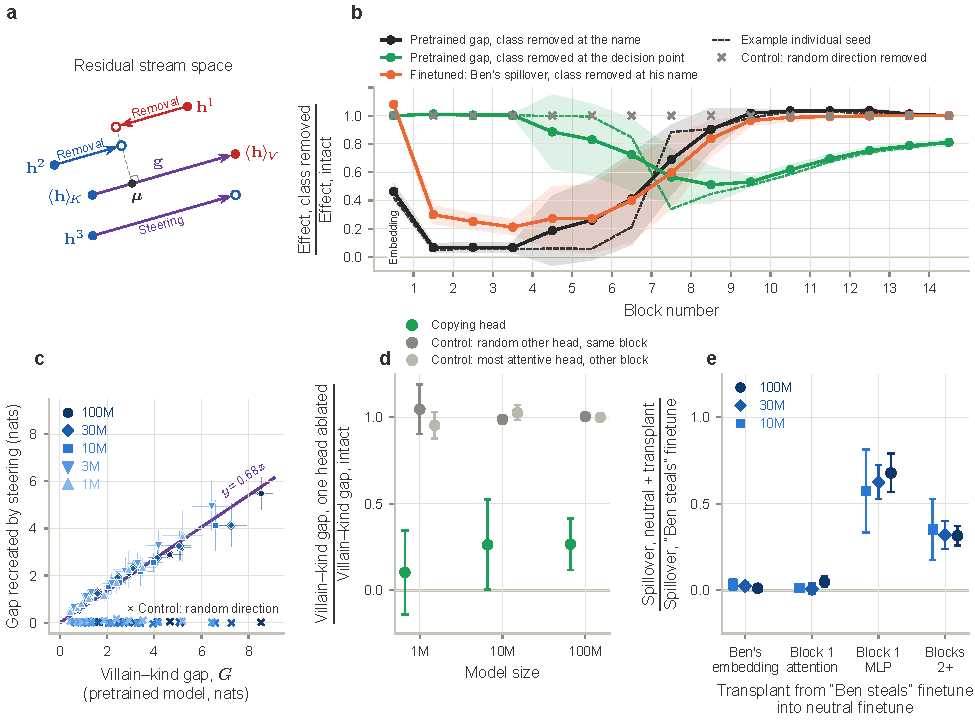
\includegraphics[width=\textwidth]{fig6_mechanism.pdf}
  \caption{
    \textbf{Interventions on activations and weights.}
    ``Villain/kind names'' at $z=0$ (\textbf{c}: $0 \le z \le 0.5$).
    Bands and error bars: 95\% CI over 8 seeds.
    Gap: villain-kind gap, as in \cref{fig:readout} (over all four acts).
    Spillover: onto ``lie,'' ``cheat,'' and ``tease'' after the ``Ben steals'' finetune (see \cref{fig:test}).
    \panel{a} Illustration of the interventions in \textbf{b} and \textbf{c}.
    $\langle\mathbf{h}\rangle_V$ and $\langle\mathbf{h}\rangle_K$: the mean residual streams of villain-name and kind-name items after a given block, at one token (\textbf{b}: the name or the decision point).
    $\mathbf{g}$: the class vector (\cref{eq:class-dir}).
    $\boldsymbol{\mu}$: the mean over all items. $\mathbf{h}^1$--$\mathbf{h}^3$: example items.
    Removal: set an item's component along $\mathbf{g}$ to match $\boldsymbol{\mu}$ (\cref{eq:remove}).
    Steering: add $\mathbf{g}$ to a kind name's embedding (\cref{eq:steer}).
    \panel{b} Locating the class (villain or kind) in the residual stream (100M models).
    The removal happens at one point in the residual stream: after the embedding, or after a transformer block, each with its own $\mathbf{g}$ (points sit between blocks).
    At the name: every token of every mention of the relevant character's name.
    At the decision point: the last token before the endings branch, and every subsequent token in both branches, except the last token.
    Dashed: seed 3 (\cref{sec:app-mechanism}).
    Control: average over 3 random directions removed at the decision point.
    \panel{c} Steering kind names toward the villain class, one point per corpus and size.
    We add $\mathbf{g}$ (here from token embeddings, over all 24 kind names) at every mention of the name being steered.
    Gap recreated by steering: score with steering minus score without.
    Control: add a vector of random direction and the same length instead.
    Line: fit through the origin (see \cref{fig:flowbyact}c).
    \panel{d} (exploratory) Attention head ablation.
    Based on each seed's largest jump in \textbf{b} (at the name, evaluated for each model size), we identify the block with the most ``copying'' to the decision point, and further find the individual attention head that copies the most.
    We plot how much of the villain-kind gap remains when mean-ablating that ``copying head.''
    For control, we compare to mean-ablating a random other head in the same block, and the head in another block that attends most from the decision point to the name.
    \panel{e} (exploratory) Transplanting parts of a finetune. We begin with a neutral finetune and overwrite part of it with weights from the corresponding ``Ben steals'' finetune.
  }
  \label{fig:mechanism}
\end{figure}

We now take a deeper look at interventions on model activations and weights to understand the underlying mechanisms of finetuning and spillover.
Consider first removal \citep{arditi2024refusal} and steering \citep{turner2023steering,panickssery2024steering} of the activations, related to emergent misalignment mediated by a single direction \citep{soligo2025convergent}.
Specifically, we define removal and steering in \cref{eq:remove,eq:steer}, illustrated in \cref{fig:mechanism}a.
\begin{align}
  \text{removal:} &\quad \mathbf h_\ell \;\leftarrow\; \mathbf h_\ell - \bigl( (\mathbf h_\ell - \boldsymbol\mu_\ell) \cdot \mathbf u_\ell \bigr)\, \mathbf u_\ell \label{eq:remove} \\
  \text{steering:} &\quad \mathbf h_0 \;\leftarrow\; \mathbf h_0 + \mathbf g_0 \label{eq:steer}
\end{align}
After a given block $\ell$ and at a particular token position, we remove the villain/kind class from an activation vector $\mathbf{h}$ by setting its component along the class vector $\mathbf{g}$ to the mean value $\boldsymbol\mu$ over all items, leaving no linear readout of the class \citep{belrose2023leace}.
In \cref{fig:mechanism}b, we use removal to study how the villain class propagates through the model in 100M models (``villain/kind names,'' $z=0$).
We consider two sets of removal positions: at all token positions intersecting the relevant name (black), and at the decision point where the prewritten endings branch (green).
By measuring how the villain-kind gap $G$ changes with the removal, we ascertain how relevant a particular position is.
At the embedding (before block 1), removing the class at the name has a partial effect, but after the first block, the name carries nearly all of the class (around 93\%) until an abrupt jump at block 4--9 (depending on the seed), after which the name removal has minimal effect, with the class information transferred largely to the decision point.
Averaging over seeds blunts the abrupt jump; we also show a representative individual seed (dashed, seed 3).
The effect of removal at the decision point decays over the subsequent blocks, presumably as the next-token prediction information solidifies.
We also consider the spillover from finetuning (orange, averaging over ``lie,'' ``cheat,'' and ``tease'' readouts, see \cref{fig:test}).
Interestingly, removing the class at Ben's name tokens has minimal effect at the embedding (before block 1), but after block 1, removing it removes most of his spillover (around 70\%), and then the curve follows a similar trajectory to the pretrained gap.
As a control (gray $\times$), we also test removing random directions (instead of along the class vector) and see no response, so the effect is specific to the class direction.
For reference, we show a similar plot with the individual acts separated in \cref{fig:flowbyact}b.
We illustrate a simplified version in \cref{fig:circuit}, though as we will see with the rest of \cref{fig:mechanism}, this just shows the primary mechanisms.
% Figure 7: the circuit (schematic). Drawn by dramatis scripts/paper_fig.py (make figures).
\begin{figure}[tbp]
  \centering
  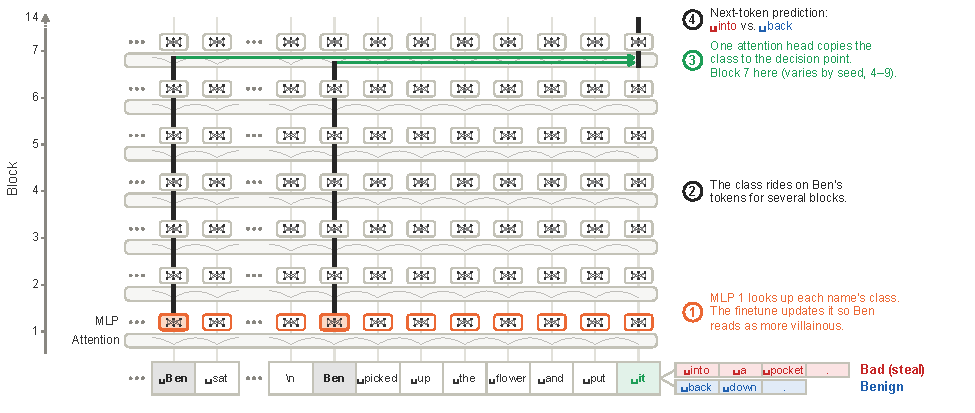
\includegraphics[width=\textwidth]{fig7_circuit.pdf}
  \caption{
    \textbf{Finetuning and ``copying head'' mechanisms.} (exploratory)
    Illustration of \cref{fig:mechanism} (100M, seed 3).
    Bottom: Ben's stealing item from \cref{fig:readout}, branching into the bad and benign endings.
    Transformer blocks stack upward.
    Faint vertical lines: each token's residual stream.
    Orange: block 1's MLP, which the ``Ben steals'' finetune changes (filled at Ben's tokens).
    Green: the decision point's first token.
  }
  \label{fig:circuit}
\end{figure}


Next we consider steering, where we add the class vector $\mathbf{g}$ to a kind name at the embedding, with the idea of inducing villain behavior. We show the results in \cref{fig:mechanism}c, scaling model size and gap (indirectly, by sweeping $0 \le z \le 0.5$).
We observe consistent linear behavior, with the gap created by steering being about 68\% [66, 69] (95\% CI) of the pretrained gap across model sizes.
For reference, we plot the models separately in \cref{fig:flowbyact}c.
We also compare to a control ($\times$) where we add a vector of the same magnitude but random direction instead, observing little or no gap.

Finally, we move to broader interventions.
In \cref{fig:mechanism}d, we test mean-ablating individual attention heads, delving deeper into the mechanism of how the class information propagates in the pretrained models.
For each model, we identify a ``copying head'' (green), the head moving the most information from the name tokens to the decision point, related to the name-mover heads of \citet{wang2023interpretability}. Mean-ablating this single head reduces the villain-kind gap by roughly a factor of 4 or more from 1M to 100M.
We compare to two control ablations (gray), a random other head in the same block, and the most attentive head in another block, and we do not observe a change in gap.
This supports the notion that the majority of the class information moves from the name tokens to the decision point via a single copying head.
In \cref{fig:mechanism}e, we return to the finetuned models, transplanting parts from the ``Ben steals'' finetune into a neutral finetune \citep[cf.][]{feng2025extractive} to see where there is substantial change, as measured by additional spillover.
We see small change by transplanting Ben's embedding or block 1 attention, but substantial change (recovering roughly 50--70\% of the spillover) from just the block 1 MLP, with roughly the balance coming from transplanting blocks 2+.
This highlights the block 1 MLP as the main site of the finetune's change. In the pretrained models, the same MLP looks up each name's class \citep{geva2021transformer}, which is why removing the class at the embedding leaves part of the gap (\cref{fig:mechanism}b), and steering the embedding recreates only about two-thirds of the gap (\cref{fig:mechanism}c).

Overall, we find a credible explanation for how most of the class information propagates from the name tokens, is augmented by the block 1 MLP, and transfers to the decision point primarily through a single attention head, a small-scale version of the factual-recall route in larger models \citep{meng2022locating,geva2023dissecting}.
Additionally, the finetune produces spillover mainly by adjusting the block 1 MLP's output for Ben's name, reusing machinery built in pretraining \citep{prakash2024finetuning,jain2024mechanistically}.

\subsection{Inferring character from context}
\label{sec:incontext}
% Figure 8: the in-context character. Drawn by dramatis scripts/paper_fig.py (make figures).
\begin{figure}[tbp]
  \centering
  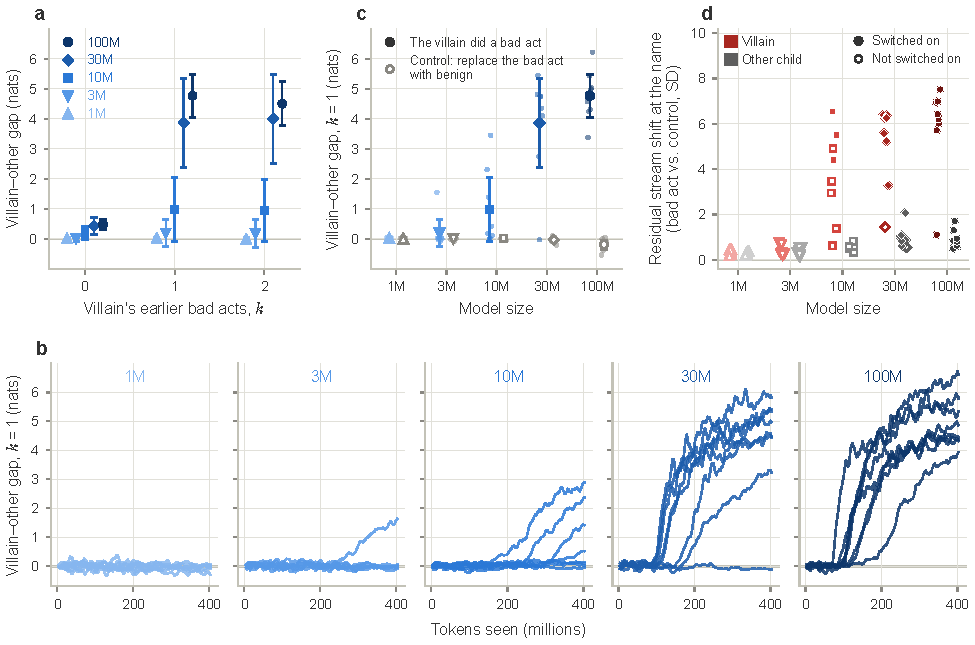
\includegraphics[width=\textwidth]{fig8_incontext.pdf}
  \caption{
    \textbf{Inferring character from context.}
    Pretraining with the coin-flip corpus (random names, coin-flip roles; see \cref{fig:design}c). Error bars: 95\% CI over 8 seeds.
    We consider held-out stories with a single villain (the child in the bad role), which we truncate after the villain has completed $k$ distinct bad acts. Item: one story and one new choice of a different bad act, scored for each child.
    For scoring prewritten endings (\textbf{a}--\textbf{c}), we average over ``steal,'' ``cheat,'' and ``tease,'' excluding ``lie'' (prewritten ``lie'' endings are a weak readout; see text).
    \panel{a} Inferred villain role vs. number of earlier bad acts and model size.
    Villain-other gap: the villain's score minus the other child's on the same item (\cref{fig:readout}a).
    Each point is the gap averaged over items, 3 acts, and 8 seeds.
    $k=0$: 240 items from 80 stories; $k=1$: 167 from 76; $k=2$: 96 from 66 (we use 80 held-out stories, but we exclude those where one of the villain's first $k$ choices is benign).
    \panel{b} (exploratory) Onset of the villain-other gap during pretraining.
    Gap at $k=1$, measured every 160k tokens during pretraining (running mean, 8.4M-token window).
    Each trace is an individual seed (8 per model size).
    25 items from 12 stories (subset of \textbf{a}).
    \panel{c} (exploratory) Control on story structure.
    Gap at $k=1$, as in \textbf{a}. Small points: individual seeds.
    Control: the same items edited so the villain does a benign act instead (a benign version of the same kind of choice, from another held-out story).
    \panel{d} (exploratory) Checking the residual stream.
    Shift in the residual stream (after the last block) at the name of the child being tested, in the setup of the new choice, compared to the control (as in \textbf{c}, same items). Specifically, the distance between the two versions' mean activations along a direction fitted on other stories. In units of the standard deviation (SD) across stories.
    Red: villain tested; gray: other child tested.
    Points: individual seeds.
    Switched on: the seed's final gap at $k=1$ (\textbf{a}) exceeds 0.5 nats.
  }
  \label{fig:incontext}
\end{figure}

Now we consider whether models can predict bad behavior based just on previous acts in the context window, where name identities in the pretraining data are uninformative; larger language models can infer a character or persona from context \citep{andreas2022agent,kim2026read}.
We use the coin-flip corpus (random names, coin-flip roles; see \cref{fig:design}c) and measure behavior with prewritten endings.
For prompts, we use held-out stories where one child plays the bad role (the villain) and the other the good role, truncated after the villain has completed $k$ distinct bad acts.
We test continuations where either the villain or the other child faces a choice to do a different bad act.
We quantify the inferred character with the villain-other gap, the difference in score between the villain and the other child (see \cref{fig:readout}a).

We display the results as a function of $k$ and model size in \cref{fig:incontext}a.
At $k=0$, we expect zero gap, as the villain has not yet done anything bad. We do see a small increase in gap with model size (about 0.5~nats for 30--100M). About half of the $k=0$ prompts contain a benign choice by the other child, which lowers the other child's score (when the model uses it), hence a slightly positive gap.
Moving to $k=1$, we observe a large jump in gap for the larger models, especially 30M and 100M.
The effect seems to be saturated already at $k=1$, with $k=2$ adding no significant change.
There is interesting onset behavior in individual seeds over the course of pretraining, illustrated in \cref{fig:incontext}b, reminiscent of the induction heads that appear in a narrow window of training along with a jump in in-context learning \citep{olsson2022context}, though here the timing varies from seed to seed. The seeds begin ``off,'' not registering any appreciable villain-other gap.
At 1M, they all remain that way through all 400M pretraining tokens.
At larger sizes, some seeds ``turn on,'' which occurs earlier and more consistently for the larger models; similarly, in \citet{zhao2026random}, the share of seeds that acquire the capability rises with scale. We define a seed as ``on'' when its gap at $k=1$ exceeds 0.5~nats.
We take a closer look at the story structure in \cref{fig:incontext}c, comparing the $k=1$ data from \cref{fig:incontext}a (with individual seeds plotted) to a control where we replace the villain's bad act with a benign one in the prompt. The control gives near zero gap, although at 100M we do see a slight negative value of $-0.19$ [$-0.35$, $-0.03$] (95\% CI), much smaller than the observed 5~nat gap. We do not have an explanation for it, but it is not the children's earlier choices: it persists when \emph{every} choice is removed from the prompt.

Finally, we examine the residual stream.
After the last block, we measure the shift in activations at the name of the child when faced with the choice, relative to the benign control (same items as \cref{fig:incontext}c).
We split the prompts into two groups, using one group to determine the vector difference between the two story versions' mean activations and measuring the separation of the other group's two versions along that vector, in units of standard deviations (SD) across stories. We swap the groups and average (cross-validation).
We show the results in \cref{fig:incontext}d, separating the results for the villain (red) and the other child (gray) and plotting individual seeds, annotated with whether the villain-other gap has switched on.
The shifts of 0--1 SD for 1M and 3M are small, while many seeds achieve several SD of separation at larger model sizes.
Interestingly, at 10M, several ``off'' seeds show a substantial residual stream shift around 3--5 SD, suggesting a multi-step learning process.
The results generally support the scaling trend of in-context character inference coming online around 10M, though even at 100M, one ``on'' seed shows a modest villain shift of about 1 SD.

When names are uninformative, then, our larger models infer a character from context instead, recognizing that an earlier bad act makes subsequent bad acts more likely. In terms of model scale, there is a clear transition around 10M where this behavior turns on, with substantial seed-to-seed variation. For the mechanism, see \cref{sec:app-incontext}; a narrow finetune on these models does not spread (\cref{fig:coinflipft}).

\section{Research lessons}
\label{sec:lessons}

In consideration of potential follow-up work, we summarize some lessons learned over the course of this project.

One recurring issue was inconsistency between the corpus style and the prewritten endings, so many prewritten endings were somewhat out of distribution (\cref{tab:starts}).
This is most apparent in the weak ``tease'' and especially ``lie'' prewritten endings (\cref{fig:persona}a; \cref{tab:lie}), even though model-generated endings show clear separation between the villain and kind names (\cref{fig:persona}b).
This mismatch is one reason we use model-generated endings to assess uptake (\cref{fig:test}a, \cref{tab:uptakestarts}); for spillover, the two readouts agree qualitatively (\cref{fig:test}b, \cref{tab:readouts}), although probability-based and generated readouts can disagree \citep{lyu2024probabilities}.
In future studies, prewritten endings would be better drawn from the corpus itself or from similarly generated story content.
Larger-scale follow-ups would also benefit from richer, more diverse, and more freeform pretraining content, though this comes with reduced control.

Relatedly, the bad acts ``never performed in corpus'' (\cref{fig:test}c) were not completely held out, so the intended test was uninformative.
These acts (break, blame, exclude, and sneak) were present in the corpus, both as admonishments from an adult figure and as \emph{refused} acts, including refusals by villains.
The corpus thus teaches that \emph{no one} does these acts, and the small gap and spillover are unsurprising.
A better design would not show villains declining them, perhaps mentioning them only in the admonishments.
Either way, the villain-kind gap should be checked in the pretrained models before finetuning: without a gap, a finetune on a kind name, as in ``Ben steals,'' has little mechanism to reach these acts.

Two smaller matters also deserve more care. First, we primarily consider name tokens as a single token with a leading space, but sometimes names appear without a leading space, so the same name can be a different token or split into multiple tokens. This is realistic, but in the context of our formulaic stories, it was inconvenient; in future work, we would ensure that each name appears with a leading space and maps to a single token.
Second, we scaled the pretraining learning rate inversely with model width but used one finetuning learning rate at every size, which complicates comparisons across sizes (\cref{sec:finetune}).

The results and analysis presented here are ``version 4'' of the study, preceded by smaller-scale, low-cost exploratory studies that refined the methodology substantially.
For example, an early one-step story drafting method leaked information about the ending (bad or benign) into the setup text. Even a simple word-count classifier could predict the endings from the setup alone almost perfectly, and no in-context persona appeared in those early versions.
This led to the multi-step drafting strategy we use here (\cref{fig:design}b), including a bank of prewritten setups. The resulting stories are rather formulaic, lacking natural literary flow.
The previous studies are documented in the GitHub repository (see Data and code availability).

\section{Discussion}
\label{sec:discussion}

Our study examines character formation in miniature in the context of emergent misalignment.
In our results, a narrow finetune spills over to other bad behaviors when pretraining has tied behavior to a persistent identity.
Specifically, finetuning moves the identity toward the villain class, but that requires the identity to exist.
This is aligned with the persona-selection explanation of emergent misalignment \citep{marks2026persona}, though a step removed from chat models and agents, where the assistant persona itself is the relevant character.
In our setting, the pretraining corpus determines whether the finetune spreads, a link proposed by \citet{soligo2026emergent} but left open.
There are also alternative explanations for emergent misalignment, which we do not test, such as \citet{li2026emergent}, who predict the spread from the base model's distance to the training data.

Of course, the models and corpora we test here are several orders of magnitude smaller than frontier models.
Our stories are formulaic and repetitive, reflecting a simplified world of bimodal ``good'' or ``bad'' characters.
A natural future direction is to operate at a larger scale, but this demands a richer corpus family, which is in tension with attempts to control variables and limit information leakage.
Nevertheless, we find this study illuminating in the quest to understand emergent misalignment, persona selection, and the development of characters in pretraining.

% End matter: two unnumbered paragraphs after the Discussion.
\paragraph{Data and code availability.}
Code is available at \url{https://github.com/kjsatz/dramatis} (MIT license), covering story generation, training, evaluation, figures, and tables, as well as previous studies and extensive notes; the repository also contains the source of this manuscript (CC-BY-4.0 license).
Corpus, finetuning, and evaluation data are available at \url{https://huggingface.co/datasets/kjsatz/dramatis-v4-data} (CC-BY-4.0 license).
Training runs including model checkpoints are available at \url{https://huggingface.co/kjsatz/dramatis-v4-runs} (MIT license).
To rebuild, clone the GitHub repository, download data with \repofile{scripts/download.py}, and run \texttt{make figures} and \texttt{make tables} to recreate the figures and tables.

\paragraph{Use of AI.}
We made substantial use of Claude Code as a research assistant. Claude wrote most of the code (the model and training loop were written by K.S. for educational purposes). Claude ran and monitored the experiments, performed literature searches, drew the figures with substantial feedback and design choices from K.S., and fact-checked the manuscript. Gemini 4 Argon was also used for iterating designs for \cref{fig:design,fig:readout} and for reviewing the manuscript.

Gemma 4 26B wrote story scenes and endings, with Claude curating the prewritten setups (from Gemma drafts) and writing the openings, closings, and filler text. Claude wrote the prewritten endings, reviewed by K.S.
Gemini 3.8 Flash judged the model-generated endings.

K.S. directed the study, made its decisions, and wrote the text with significant editing and assistance from Claude. K.S. is responsible for the contents of this manuscript.


\bibliographystyle{plainnat}
\bibliography{refs}

% The appendix starts on a fresh page, so no appendix float lands among the references
\clearpage
\appendix
% \cref prints the appendix's sections and subsections as "Appendix A.1", not "Section A.1"
\crefalias{section}{appendix}\crefalias{subsection}{appendix}
% Everything numbered in the appendix carries an A prefix (Figure A1, Table A1, Equation (A1)), counted afresh;
% the \theH... versions give hyperref distinct link targets from the main text's.
\setcounter{figure}{0}\setcounter{table}{0}\setcounter{equation}{0}
\renewcommand{\thefigure}{A\arabic{figure}}\renewcommand{\theHfigure}{A\arabic{figure}}
\renewcommand{\thetable}{A\arabic{table}}\renewcommand{\theHtable}{A\arabic{table}}
\renewcommand{\theequation}{A\arabic{equation}}\renewcommand{\theHequation}{A\arabic{equation}}
\section{Appendix}
\label{sec:appendix}
\suppressfloats[t]  % no float above the Appendix heading on its own page

\subsection{Readouts and statistics}
\label{sec:app-readouts}

% Table A1: how bad endings start. Body generated by dramatis scripts/paper_tables.py (make tables).
\begin{table}[tbp]
  \centering
  \small
  \caption{
    \textbf{How bad endings start.}
    In the corpus: every bad ending of the four performed acts.
    Model-generated: using pretrained $z=0$ models, 1M--100M, 3 seeds pooled, villain names, restricted to endings judged as ``bad.''
    Prewritten: the 64 bad endings (4 acts, 16 items per act).
  }
  \label{tab:starts}
  \begin{tabular}{lrrrr}
\toprule
 & \multicolumn{3}{c}{The ending starts with} & \\
\cmidrule(lr){2-4}
 & the child's name & ``While'' or ``When'' & a quote & $n$ \\
\midrule
\multicolumn{5}{@{}l}{\emph{In the corpus, as written}} \\
Steal & 18\% & 82\% & 0\% & 559{,}061 \\
Cheat & 59\% & 40\% & 0\% & 560{,}648 \\
Tease & 0\% & 0\% & 100\% & 559{,}839 \\
Lie & 0\% & 0\% & 100\% & 560{,}452 \\
\midrule
\multicolumn{5}{@{}l}{\emph{Model-generated endings, villain names}} \\
Steal & 9\% & 91\% & 0\% & 953 \\
Cheat & 59\% & 41\% & 0\% & 924 \\
Tease & 0\% & 0\% & 100\% & 922 \\
Lie & 0\% & 0\% & 100\% & 959 \\
\midrule
Prewritten endings, all four acts & 100\% & 0\% & 0\% & 64 \\
\bottomrule
\end{tabular}

\end{table}

% Table A2: the two readouts compared. Body generated by dramatis scripts/paper_tables.py (make tables).
\begin{table}[tbp]
  \centering
  \small
  \caption{
    \textbf{Comparing prewritten and model-generated readouts.}
    ``Ben steals'' at 10M. Mean with 95\% CI over 8 seeds.
    At $z=1$, the prewritten readout does not see the uptake; see \cref{tab:uptakestarts}.
  }
  \label{tab:readouts}
  {\setlength{\tabcolsep}{3pt}\begin{tabular}{@{}lrrrr@{}}
\toprule
 & \multicolumn{2}{c}{Uptake on ``steal''} & \multicolumn{2}{c}{Spillover onto ``cheat'' and ``tease''} \\
\cmidrule(lr){2-3}\cmidrule(lr){4-5}
Corpus & model-generated & prewritten & model-generated & prewritten \\
 & (pts) & (nats) & (pts) & (nats) \\
\midrule
Villain/kind names, $z=0$ & +85 [78, 92] & +6.65 [5.38, 7.93] & +44 [30, 58] & +1.98 [1.37, 2.59] \\
Specialist villain names, $z=0$ & +84 [77, 91] & +4.61 [3.42, 5.81] & +13 [8, 17] & +0.64 [0.35, 0.92] \\
Villain/kind names, $z=1$ & +68 [53, 83] & $-$0.09 [$-$0.27, 0.09] & +1 [$-$8, 9] & $-$0.02 [$-$0.06, 0.01] \\
\bottomrule
\end{tabular}}

\end{table}

% Table A3: the z = 1 uptake by how the ending starts. Body generated by dramatis scripts/paper_tables.py (make tables).
\begin{table}[tbp]
  \centering
  \small
  \caption{
    \textbf{Uptake dependence on ending start.}
    Villain/kind names at $z=1$ (names are random), 10M.
    Uptake measured with model-generated endings after the ``Ben steals'' finetune, on ``steal'' items, 8 seeds pooled.
    Theft rate: share of model-generated endings the judge labeled ``bad.''
    $n$: how many endings start this way.
  }
  \label{tab:uptakestarts}
  \begin{tabular}{lrrrr}
\toprule
 & \multicolumn{2}{c}{Ben} & \multicolumn{2}{c}{Other kind names} \\
\cmidrule(lr){2-3}\cmidrule(lr){4-5}
Ending starts with & Theft rate & $n$ & Theft rate & $n$ \\
\midrule
``While'' & 97\% & 113 & 96\% & 57 \\
the child's name & 33\% & 15 & 10\% & 389 \\
another way & --- & 0 & 0\% & 2 \\
\midrule
All & 90\% & 128 & 21\% & 448 \\
\bottomrule
\end{tabular}

\end{table}

% Table A4: the lie items. Body generated by dramatis scripts/paper_tables.py (make tables).
\begin{table}[tbp]
  \centering
  \small
  \caption{
    \textbf{The prewritten ``lie'' items.}
    Items classified by style, \emph{denial} (which is consistent with the corpus) and \emph{blame}.
    Gaps computed for $z=0$ models, averaged over 8 seeds and the items in each style grouping.
    For context, in model-generated endings (10M, after the neutral finetune), villain names exclusively use denial ($n=128$).
  }
  \label{tab:lie}
  \begin{tabular}{llcw{c}{5.5em}w{c}{5.5em}}
\toprule
 & & & \multicolumn{2}{c}{Villain-kind gap, $G$ (nats)} \\
\cmidrule(lr){4-5}
Bad ending style & Example & Items & 10M & 100M \\
\midrule
Denial & \emph{``I did not knock it over at all.''} & 2 & +15.3 & +15.0 \\
Blame & \emph{``The wind [or a cat] knocked it over.''} & 14 & $-$1.3 & $-$1.0 \\
\bottomrule
\end{tabular}


\end{table}


\subsubsection{Model-generated endings}
\label{sec:app-readouts:generated}
For prompts, we use the first 4 of each act's 16 prewritten setups, truncated when the choice is presented.
We sample up to 60 tokens at temperature 1 (no top-$k$).

The judge LLM is Gemini 3.8 Flash, thinking off, temperature 0, with JSON output.
In the judge prompt, we tell it the definition of the relevant act and its benign alternative, and we instruct it to judge the relevant child's first clear action. It is not told anything about the name's class.
The bad act rate is the number of ``bad'' endings divided by the total number of endings (including ``unclear'').
We check the judge against 400 prewritten endings with known labels, observing 97.5\% agreement.
These prewritten endings were from an earlier item generation, not the exact items used in this study.

The total cost of judging the 82{,}400 samples used here was about \$52.

\subsubsection{Prewritten endings}
\label{sec:app-readouts:prewritten}
The scores $s$ are sums of $\log(p)$ over the ending's tokens (not divided by the number of tokens).
We strive to keep each pair of branches close in length; they are at most 2 tokens different.
Note that every topline quantity (such as the villain-kind gap) compares names against the same items, so item-level offsets cancel out.

To evaluate the villain-kind gap $G$ on a particular model and type of act (e.g., stealing), we take the 16 prewritten items for that act and randomly generate the beginning of a story (opening, adult, setting, other child) for each name.
Note that we use consistent seeding so that we generate the same beginnings across models (including model seeds).
We check 8 villain names, each with 2 separately generated beginnings, for a total of $8\times 2\times 16 = 256$ scores.
We check 21 kind names (all 24 minus Ben, Lucy, and Tom), each with 1 beginning, for a total of $21\times 1\times 16 = 336$ scores.
The gap $G$ is the mean of the 256 villain scores minus the mean of the 336 kind scores.

\subsubsection{Confidence intervals}
\label{sec:app-readouts:intervals}
We compute confidence intervals (CI) for the mean over seeds using t intervals.
Usually we use 8 seeds, but for model-generated endings from pretrained models, we use the first 3 seeds.
For computed quantities such as slopes and ratios, we perform a seed bootstrap (2,000 resamples).

\subsection{Finetune detail}
\label{sec:app-finetune}

% Figure A1: Figure 4a split into Ben's and the other kind names' changes. Drawn by dramatis scripts/paper_fig.py (make figures).
\begin{figure}[tbp]
  \centering
  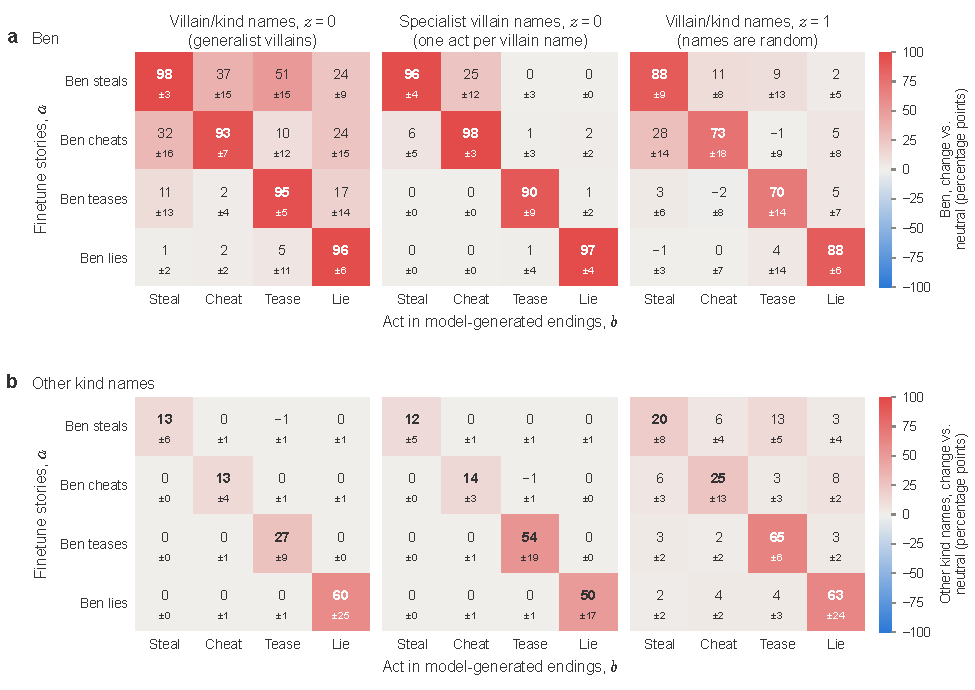
\includegraphics[width=\textwidth]{figA1_finetune_parts.pdf}
  \caption{
    \textbf{Finetune effects on Ben and other kind names.}
    See \cref{fig:test}a caption.
    \cref{fig:test}a shows the difference between Ben's behavior change (under a finetune focusing on Ben) and the other kind names. Here, we show these separately.
    Based on model-generated, LLM-judged endings.
    Means over 8 seeds, 95\% CI.
    \panel{a} Change in how often Ben does each act after the specified Ben finetune, relative to a neutral finetune.
    \panel{b} Change in how often other kind names (mean over 7 names) do each act after the specified Ben finetune, relative to a neutral finetune.
  }
  \label{fig:testparts}
\end{figure}

In \cref{fig:testparts}, we show an alternative version of \cref{fig:test}a, where we split apart the shift of Ben's behavior (\cref{fig:testparts}a) and the shift of other kind names' behavior (\cref{fig:testparts}b). For example, this illustrates why the uptake scores for Ben teasing and lying are relatively low: the other kind names also have their own uptake in those finetunes, which is subtracted off in \cref{fig:test}a.

% Figure A2: the paired-act villain names matrix, and spillover for every corpus. Drawn by dramatis scripts/paper_fig.py (make figures).
\begin{figure}[tbp]
  \centering
  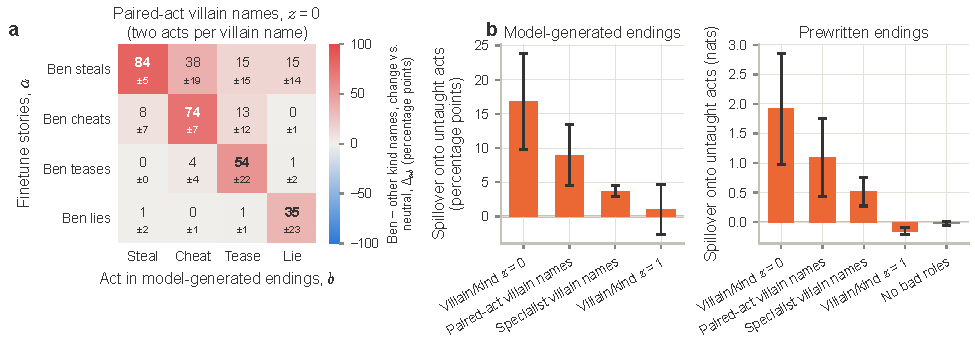
\includegraphics[width=\textwidth]{figA2_all_corpora.pdf}
  \caption{
    \textbf{Finetunes on additional corpora.}
    See \cref{fig:test} caption.
    We include additional corpora, ``paired-act villain names'' and ``no bad roles'' (see text).
    Means over 8 seeds, 95\% CI.
    \panel{a} Same plot as \cref{fig:test}a, for ``paired-act villain names.''
    \panel{b} Same plot as \cref{fig:test}b, adding entries for ``paired-act villain names'' and ``no bad roles.''
  }
  \label{fig:allcorpora}
\end{figure}

We tested another corpus, ``paired-act villain names,'' which is not included in the main text (see \cref{tab:corpora}).
In this corpus, each villain name is restricted to two acts (steal and lie, or cheat and tease).
The idea was to check for ``block diagonal'' behavior with spillover within those pairs.
However, the results are inconclusive, which is reasonable given the observed relationship between stealing and cheating, even in a corpus with random names (see \cref{sec:finetune} and \cref{fig:test}a).
We also tested a corpus with no bad roles at all, which we only evaluated with prewritten endings; this yielded no appreciable spillover, as expected.
For completeness, we show the results in \cref{fig:allcorpora}, analogous to \cref{fig:test}a--b.

\subsection{Mechanism detail}
\label{sec:app-mechanism}
% Figure A3: Figure 6b per act at 100M, and Figure 6c per model size. Drawn by dramatis scripts/paper_fig.py (make figures).
\begin{figure}[tbp]
  \centering
  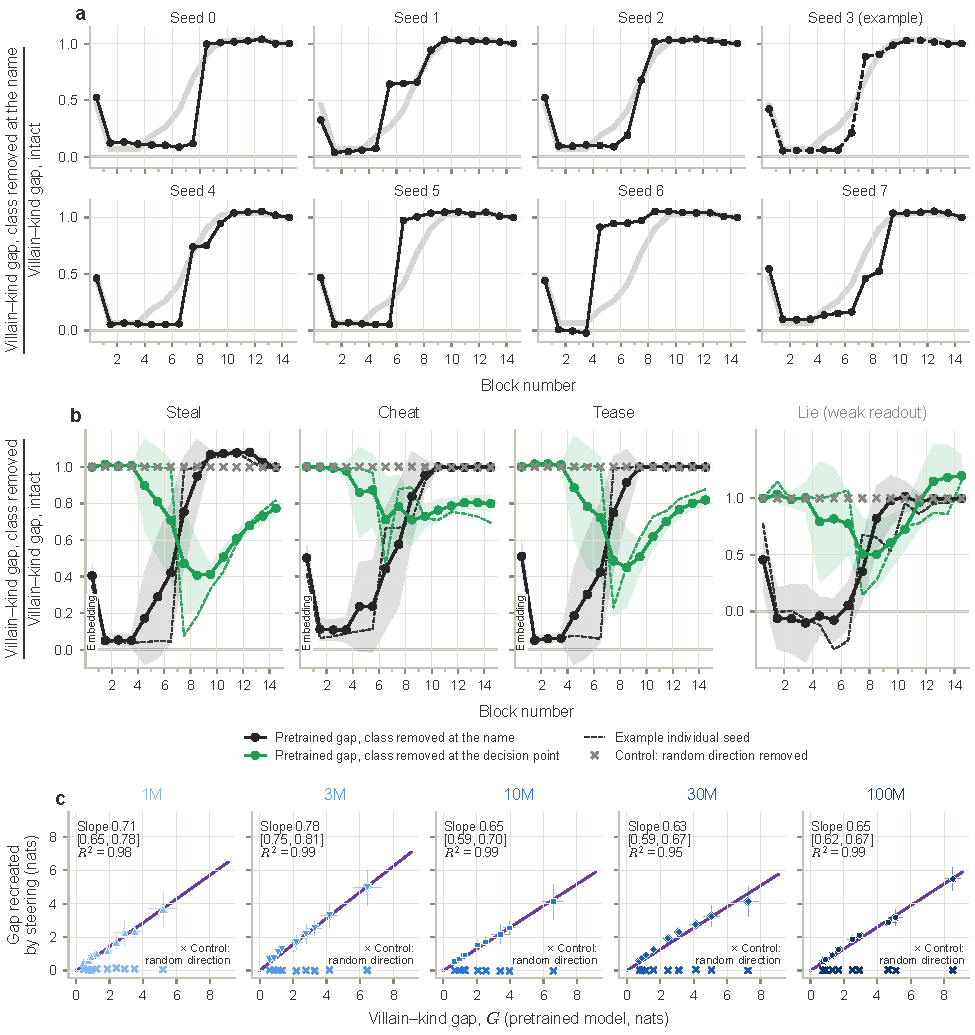
\includegraphics[width=\textwidth]{figA3_flow_by_act.pdf}
  \caption{
    \textbf{Interventions on activations, separated by seed, act, and model size.}
    We split out aggregated plots from \cref{fig:mechanism} for reference.
    \panel{a} See \cref{fig:mechanism}b, specifically the pretrained gap with the class removed at the name.
    Gray: mean over seeds (as plotted in \cref{fig:mechanism}b).
    Black: each individual seed. We chose seed 3 (dashed) as a representative example in \textbf{b} and \cref{fig:mechanism}b (see text).
    \panel{b} See \cref{fig:mechanism}b, which was averaged over all four acts.
    Here, we plot them separately.
    Note wider y range for ``lie'' due to the broader confidence intervals.
    Pretrained gap only (no finetunes shown).
    \panel{c} See \cref{fig:mechanism}c. Here we split the data into separate plots for each model size, including separate linear fits through the origin.
    Under the slope annotation, we list 95\% CI for the slopes and $R^2$ from regression.
  }
  \label{fig:flowbyact}
\end{figure}

In \cref{fig:mechanism}b, we chose seed 3 as representative, because its largest jump is at the median block number and size, and its shape is typical (seed 4 is also at the median jump block number and size).
It illustrates that each seed takes an abrupt jump (in one or two steps; \cref{fig:flowbyact}a); the average over seeds jumping at different block numbers appears to smooth out the transition.

\cref{fig:mechanism}b averages the pretrained gap over the four bad acts. In \cref{fig:flowbyact}b, we plot them separately for reference. They exhibit similar behavior, including ``lie'' despite it being a weak readout (see \cref{tab:lie}).

\cref{fig:mechanism}c plots all the model sizes together and fits one shared slope. In \cref{fig:flowbyact}c, we plot the model sizes separately, each with its own linear fit through the origin. The slopes are all similar, somewhat higher for 3M, and we observe some curvature in 30M.

\subsection{Details on inferring character from context}
\label{sec:app-incontext}

% Figure A4: the "Ben steals" finetune on the coin-flip corpus. Drawn by dramatis scripts/paper_fig.py (make figures).
\begin{figure}[tbp]
  \centering
  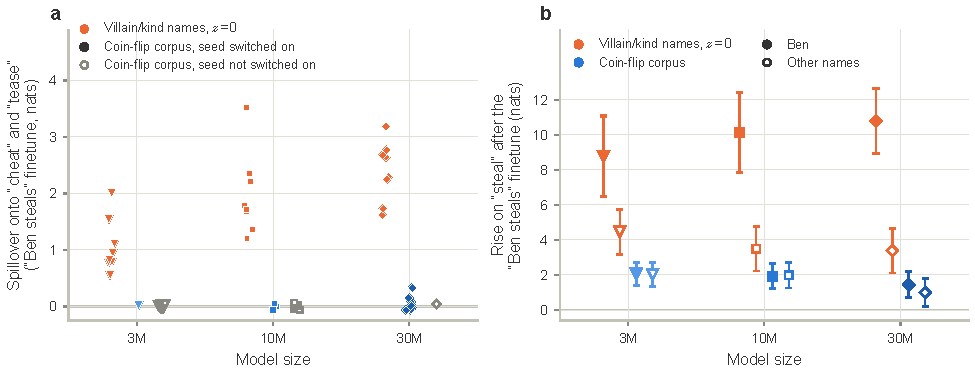
\includegraphics[width=\textwidth]{figA4_finetune_coinflip.pdf}
  \caption{
    \textbf{Finetune on the coin-flip (random names) corpus.} (exploratory)
    Measured at 3M, 10M, and 30M, with prewritten endings.
    \panel{a} Checking for spillover in the coin-flip corpus.
    \cref{fig:graded}d shows the same spillover normalized to the gap.
    Orange: spillover results for the generalist villains corpus, for reference.
    Individual seeds plotted.
    Switched on: villain-other gap at $k=1$ exceeds 0.5 nats (as in \cref{fig:incontext}d).
    \panel{b} Checking for uptake in the coin-flip corpus.
    Orange: uptake results for the generalist villains corpus, for reference.
    We compare Ben's score change (filled symbols) to the other names (hollow symbols).
    Mean over 8 seeds, 95\% CI.
  }
  \label{fig:coinflipft}
\end{figure}

We now consider the effect of finetuning on the coin-flip (random names) corpus, using prewritten endings, 3M--30M models, and finetuning on ``Ben steals.''
In \cref{fig:coinflipft}a, we check for spillover after finetuning.
Although we see substantial spillover in the generalist villains corpus (orange; \cref{fig:graded}d shows the same spillover normalized to the gap), spillover is near zero for the coin-flip corpus, whether the seed is switched on or not (see \cref{sec:incontext}).
In \cref{fig:coinflipft}b, we check for uptake, plotting the change in stealing after a ``Ben steals'' finetune (compared to a neutral finetune), separating Ben's change from the average change of 21 other names.
Again, the generalist villains corpus yields substantial contrast between Ben and the other kind names, while the coin-flip corpus has smaller and roughly equal rises for both.
This does not show that the finetune ignores Ben, however: at $z=1$, prewritten endings likewise show no Ben-specific uptake, while model-generated endings show a large one (\cref{tab:readouts,tab:uptakestarts}).

Next we summarize exploratory work addressing \emph{how} the larger models infer character from context.
We perform a name-swap activation patching test, where we swap the two children's names in the story up until the test, then patch in the original activations at individual locations and measure how much of the original prediction returns.
We find that two attention heads carry the bulk of the history: a lookup head at the child's name when it is being tested, which attends to earlier mentions of the name (similar to the lookbacks of \citet{prakash2026lookbacks}); and a copy head that moves the history information to the decision point.
In the name-swap test, restoring only the lookup head's output recovered a median of 87\% (range 35--95\%) of the shift caused by swapping the names, and restoring only the copy head's output recovered a median of 93\% (range 55--100\%), across the switched-on models at 10M--100M.
This topic is at the periphery of our scope, so we did not delve further (e.g., ablations). There is more detail in the GitHub repository, \repofile{docs/2026-09-25_REPORT_incontext_character.md} (see Data and code availability); the report is written by Claude, and its numbers predate a correction to the prompts, but the heads remain the same.


\subsection{Corpus}
\label{sec:app-corpus}
% Figure A5: one whole story. Drawn by art/fig1_design.py (make art), at its natural width (no width=).
\begin{figure}[tbp]
  \centering
  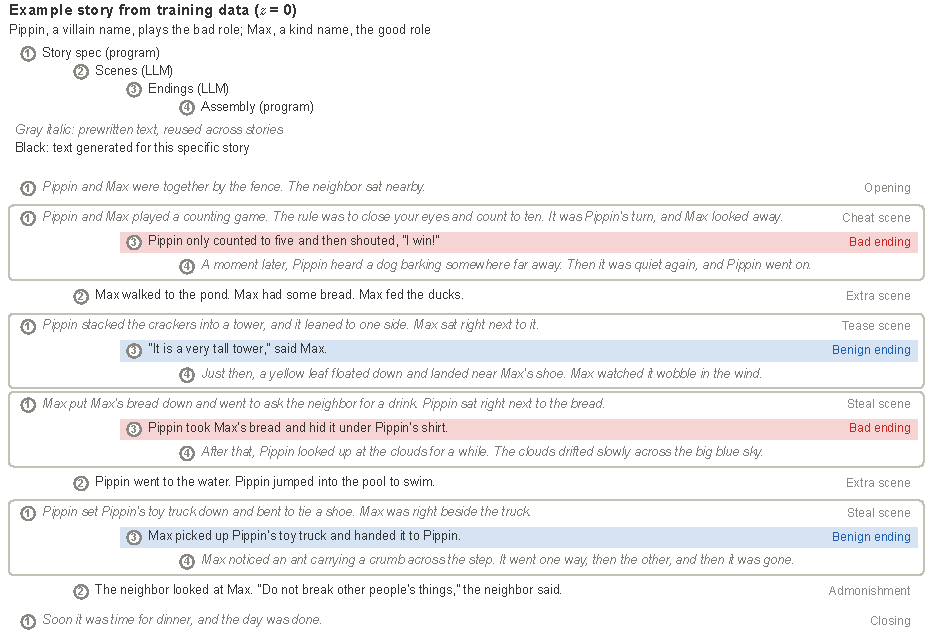
\includegraphics{figA5_story.pdf}
  \caption{
    \textbf{Example full story from training data.}
    Full story containing the example scene shown in \cref{fig:design}b.
  }
  \label{fig:story}
\end{figure}

% Table A5: the corpora. Body kept by hand in tables/tableA5_corpora.tex.
\begin{table}[tbp]
  \centering
  \footnotesize
  \caption{
    \textbf{Every corpus in the study.}
    Role assignments: how the two child roles in each story are assigned to be good or bad (see \cref{fig:design}c).
    Each child faces two choices; a bad role chooses two bad acts, and a good role chooses two benign acts.
    Varying $z$: specifically 0, 0.01, 0.02, 0.05, 0.1, 0.2, 0.3, 0.4, 0.5, 1.
    Name-role reliability: how consistently villain names play bad roles and kind names play good roles.
    Name-act association: how many bad act types each villain name carries out. For paired-act, each villain name is assigned steal/lie or cheat/tease.
    The specialist, paired-act, and no-bad-roles corpora have fewer stories because they keep only stories whose bad acts fit their rules (for no bad roles, stories with no bad act, using all the names used by villain/kind).
    Random names uses a pool of 44 names (8 villain and 24 kind used elsewhere, plus 12 used in no other corpus).
    Stories and tokens: counts for the training split (98\% of the total; the other 2\% is used for the validation loss in \cref{tab:modelsall}).
    Each model makes one pass over its corpus in pretraining.
  }
  \label{tab:corpora}
  % Table A5: every corpus. Kept by hand; story and token counts are the training splits from each corpus's recipe.json (dramatis data/corpora/v4-*/).
% "Used in", tight: Figs. 1--7, A1--A5 (cleveref's names and conjunctions set for this table only, in the group below;
% \labelcref for the appendix figures, which a single \cref would sort among the main ones)
{\crefname{figure}{Fig.}{Figs.}\crefname{table}{Table}{Tables}%
\renewcommand{\crefrangeconjunction}{--}\renewcommand{\crefpairconjunction}{, }%
\renewcommand{\crefmiddleconjunction}{, }\renewcommand{\creflastconjunction}{, }%
\setlength{\tabcolsep}{5pt}%  a little narrower than the default 6pt, so the text columns wrap less
\begin{tabularx}{\textwidth}{@{}>{\raggedright\arraybackslash}p{2.8cm} >{\raggedright\arraybackslash}X >{\raggedright\arraybackslash}p{2.3cm} >{\raggedright\arraybackslash}p{1.6cm} r r >{\raggedright\arraybackslash}p{3.0cm}@{}}
\toprule
Corpus & Role assignments & Name-role reliability & Name-act association & Stories & Tokens & Used in \\
\midrule
Villain/kind names (10 corpora, varying~$z$) & 0 or 1 bad role per story ($\tfrac12$~each) & Varies from reliable ($z=0$) to random ($z=1$) & 4 acts per villain & 981{,}278 & 409M & \cref{fig:design,fig:readout,fig:persona,fig:test,fig:graded,fig:mechanism,fig:circuit}, \labelcref{fig:testparts,fig:allcorpora,fig:flowbyact,fig:coinflipft,fig:story}; \cref{tab:starts,tab:readouts,tab:uptakestarts,tab:lie,tab:modelsall} \\
\addlinespace[4pt]
Specialist villain names & Same as villain/kind & Reliable ($z=0$) & 1 act per villain & 489{,}130 & 204M & \cref{fig:design,fig:test}, \labelcref{fig:testparts,fig:allcorpora}; \cref{tab:readouts} \\
\addlinespace[4pt]
Random names, coin-flip roles & Each role bad with probability $\tfrac12$, independently & Random & -- & 968{,}550 & 407M & \cref{fig:design,fig:incontext}, \labelcref{fig:coinflipft} \\
\addlinespace[4pt]
Paired-act villain names & Same as villain/kind & Reliable ($z=0$) & 2 acts per villain & 653{,}931 & 272M & \cref{fig:allcorpora} \\
\addlinespace[4pt]
No bad roles & All roles good & -- & -- & 490{,}639 & 203M & \cref{fig:allcorpora} \\
\bottomrule
\end{tabularx}}

\end{table}

See \cref{tab:corpora} for details about the corpora.

We generated the stories with Gemma 4 26B (\href{https://huggingface.co/google/gemma-4-26B-A4B-it}{\nolinkurl{google/gemma-4-26B-A4B-it}}, open weights) on rented H100s at a cost of about \$79. Of the 1.4M stories generated, 91\% passed programmatic validation. The corpora were programmatically assembled from those stories (\cref{fig:design}c). We also spot-checked story quality with Gemini 3.8 Flash (about \$5 to review 1{,}800 stories) and with Claude Code (50 stories).

There is substantial repetition of prewritten text across stories. Prewritten setups, openings and closings, and filler sentences (gray in \cref{fig:story}) make up about 63\% of a story's tokens, and each setup appears about 40{,}000 times in a corpus. These were written by Claude, the setups from Gemma drafts. Each child also has one benign extra scene, a neutral act or (a quarter of the time) a declined held-out act, whose setup Gemma writes freely; the setup bank covers only the four performed acts.

\subsection{Models and training}
\label{sec:app-models}
% Table A6: the models. Body generated by dramatis scripts/paper_tables.py (make tables).
\begin{table}[tbp]
  \centering
  \small
  \caption{
    \textbf{Language model parameters.}
    In the reported results, we used the 1M--100M model sizes.
    We ran experiments on the smaller 0.2M--0.8M models and release the weights, but they are not used in this paper.
    Body: all parameters except the token and position embeddings.
    Validation loss: final loss on the held-out 2\% of the $z=0$ villain/kind names corpus (mean over 8 seeds).
    See text for more details.
  }
  \label{tab:modelsall}
  \begin{tabular}{lrrrrrrr}
\toprule
 & & & & \multicolumn{2}{c}{Parameters} & & Validation loss \\
\cmidrule(lr){5-6}
Size & Layers & Width & Heads & body & total & Peak learning rate & (nats/token) \\
\midrule
0.2M & 1 & 128 & 4 & 0.20M & 0.79M & $1.8\times10^{-3}$ & 0.374 \\
0.4M & 2 & 128 & 4 & 0.39M & 0.98M & $1.8\times10^{-3}$ & 0.335 \\
0.6M & 3 & 128 & 4 & 0.59M & 1.18M & $1.8\times10^{-3}$ & 0.326 \\
0.8M & 4 & 128 & 4 & 0.79M & 1.38M & $1.8\times10^{-3}$ & 0.319 \\
\midrule
1M & 5 & 128 & 4 & 0.98M & 1.57M & $1.8\times10^{-3}$ & 0.315 \\
3M & 7 & 192 & 6 & 3.10M & 3.98M & $1.2\times10^{-3}$ & 0.301 \\
10M & 6 & 384 & 6 & 10.62M & 12.39M & $6.0\times10^{-4}$ & 0.294 \\
30M & 10 & 512 & 8 & 31.47M & 33.83M & $4.5\times10^{-4}$ & 0.289 \\
100M & 14 & 768 & 12 & 99.11M & 102.65M & $3.0\times10^{-4}$ & 0.286 \\
\bottomrule
\end{tabular}

\end{table}

See \cref{tab:modelsall} for model and training parameters.
We tokenize with byte-level byte-pair encoding (BPE) with a 4{,}096-token vocabulary trained on the TinyStories corpus from \citet{eldan2023tinystories}.
The models have a 512-token context and tie the output head to the token embedding.

We pretrain with AdamW ($(\beta_1, \beta_2)=(0.9, 0.95)$, weight decay 0.1) and clip the gradient norm at 1.
We use batches of $32\times 512$ tokens and pretrain for one full pass over the relevant corpus (roughly 25{,}000 steps for the 409M-token villain/kind names corpora).
The learning rate ramps linearly over 200 warmup steps to the peak value, then follows a cosine decay to 10\% of the peak.
We scale the peak learning rate with 1/width (see \cref{tab:modelsall}).
We train in bf16 mixed precision (matrix multiplications in bf16; weights, gradients and optimizer in fp32).

We finetune with AdamW (with a fresh optimizer state).
We do 100 steps, again over batches of $32\times 512$ tokens (1.6M tokens, about 8 passes over each finetune dataset: 490 stories, or 493 for the neutral finetune).
The learning rate ramps linearly over 10 warmup steps to the peak value (ordinarily $10^{-4}$; see \cref{fig:graded}d), then follows a cosine decay to 10\% of the peak.
We perform the neutral finetunes with the same settings.

We saved model weights for every pretrained and finetuned model.
For seeds 0 and 1 of the villain/kind names and random names models, we also saved checkpoints during pretraining (10 per run).
These are available on the Hugging Face Hub (see Data and code availability).

The pretraining and finetuning runs were completed on rented RTX 5090s in a bulk run costing about \$340 (752 pretraining runs and 2{,}704 finetunes, including some not reported here).
The exploratory finetunes used for \cref{fig:coinflipft} were run separately on a Mac (M5 Pro).


\end{document}
